\documentclass[11pt,letterpaper]{article}
\usepackage{geometry,
  multicol,
  graphicx,
  verbatim,
  fancyhdr,
  lipsum,
  lineno,
  blindtext,
  wrapfig,
authblk, hyperref}

\providecommand{\tightlist}{%
  \setlength{\itemsep}{0pt}\setlength{\parskip}{0pt}}

\title{WHPC Scholarship: Haskell Bioinformatics}
% \author{Salma Ouaakki and Calypsa McCarthy}
\author[1]{Salma Ouaakki}
\author[2]{Calypsa McCarthy}
\author[3]{Noah Jones}
\affil[1]{(Applicant) University of Florida, Herbert Wertheim College of Engineering}
\affil[2]{(Applicant) University of Florida, Institute of Food and Agricultural Sciences}
\affil[3]{(Mentor) University of Florida, College of Medicine}
\date{March 2024}

\usepackage[backend=biber,style=authoryear]{biblatex} %Imports biblatex package
\addbibresource{bibliography.bib} %Import the bibliography file

% Discuss testing the pipeline against some standard dataset/pipeline

\begin{document}
\linenumbers
\maketitle

\begin{abstract}
  There is a growing preponderance of high-dimensional data sets
  across various research fields, posing challenges related to the
  limitations of current analysis tools. Shortcomings of
  parallelizability, concurrency, and the integration of disparate
  data types have been widely acknowledged. Despite the
  prevalence of dimensionality reduction techniques in machine
  learning, a distributed version of one of the most popular
  algorithms, uniform manifold approximation and projection (UMAP),
  remains unavailable thus hindering the scalability of data
  pipelines and workflows. Additionally, while statistical analysis
  methods like R and Java are commonly used among bioinformatics
  researchers, there lacks a commercial or open-source core
  framework with features emphasizing reliability, type safety, and
  correctness guarantees.

  To address these challenges, this project proposes the development
  of a statically typed core framework in Haskell. Haskell, renowned
  for its capacity to produce bug free code, reliability, and high
  performance, presents an ideal solution. Our framework aims to
  harmonize and parallelize the analysis of datasets of high
  complexity from heterogeneous sources. By leveraging Haskell’s
  capabilities, we intend to design algorithms that are not only fast
  enough to handle large datasets, but also accessible to novice
  bioinformaticians. Moreover, the framework will provide
  significantly enhanced correctness guarantees, ensuring the
  reliability of analyses conducted within it.

   Through this endeavor, we aspire to alleviate the bottlenecks
  associated with current analysis tools and facilitate the
  exploration of high-dimensional datasets across disciplines. Our
  project underscores the importance of leveraging advanced
  programming languages and methodologies to address pressing
  challenges in data analysis and bioinformatics.

% This research proposal outlines our aim to develop a statically typed core framework in Haskell to address the challenges posed by high-dimensional datasets in bioinformatics and other research fields. By leveraging Haskell's strengths in reliability and performance, the framework seeks to provide enhanced correctness guarantees as well as harmonize and parallelize the analysis of datasets of high complexity from heterogeneous sources. Through the implementation of a distributed version of UMAP and optimization for efficiency, we intend to demonstrate that our framework alleviates the bottlenecks associated with current analysis tools and facilitates the exploration of high-dimensional datasets across disciplines.

\end{abstract}

\newgeometry{margin=.5in}
% \begin{multicols}{2}

\section{Background}

As technology advances, datasets are becoming larger and more complex,
demanding more capabilities from data analysis tools as, for example,
is the case genome-wide association studies (GWAS) where each variant
discrete variable in disease-prediction model
\parencite{huang2018high}. This in turn leads to high-dimensional data
sets, in which their variety, velocity, volume, value, and veracity
each leads to its own computatoinal challenges
\parencite{anuradha2015brief}. As datasets become larger and more
complex, so too do the problems associated with inconsistent
enforcment of data standards and bugs and interactions associated with
distributed and concurrent data processing \parencite{Schadt_2010}.

Current methods of analysis such as Principal Component Analysis (PCA)
and Multigroup Analysis (MGA), are commonly used by bioinformaticians
for dimensionality reduction; however, these techniques often fail to
differentiate distinct clusters within sets of overlapping data points
and ``face a major challenge with the rapid increase in sample size''
\parencite{yang2021dimensionality}. Despite the prevalence of
dimensionality reduction techniques in machine learning, a distributed
version of one of the most popular algorithms, Uniform Manifold
Approximation and Projection (UMAP), remains unavailable thus
hindering the scalability of data pipelines and workflows. UMAP has
been widely implemented in the field of bioinformatics as a non-linear
algorithm that can significantly reduce the dimensionality of genomics
datasets \parencite{bollon2022investigating}. Currently available UMAP
algorithms are often integrated into popular Python and R
packages. However, the bioinformatics community would be greatly
advantaged by a distributed version of UMAP because of the increased
scalability and resource utilization.

Functional programming paradigms are excellent for scaling and
parallelizing processes especially as systems grow and increase in
their complexity. Immutablity and the explicit statement of all
program effects prevent unpredictable interactions between program
threads, and lazy evaluation models permit the minimum amount of work
to be performed as it is needed. Functional languages that provide the
opportunity to choose which parts of the program are performed eagerly
or lazily offer fine control over when computatoin occurs allowing for
finer management of the executoin model.

Finally, the field of bioinformatic requires two very different
complementary skill sets: that of algorithm and program design and
that of a deep understanding of the biological problems being
addressed. It is very difficult to acquire these two domains of
expertise as they share very little common background. As a result,
many bioinformatics packages exhibit unorthodox user interfaces and
odd design choices that can make them difficult to use at best and
unintuitive to the point of misleading the user as to the nature of
the task being peformed at worst \parencite{shah2019misunderstood}. In
fact, errors are routinely found in bioinformatics packages that have
the potential to corrupt scientific findings
\parencite{chen2009innovative}. Eschewing the use of bioinformatic
tools is also a problem, as it preemptively revokes the would-be
guiderails that would have otherwise facilitated researchers in making
good experimental design decisions \parencite{biron2006pitfalls}.

We aim to address these new computational and statistical challenges
by generating a proof-of-concept bioinformatic framework within a
limited scope to demonstrate that the pure functional programming
paradigm, declarative style, and static type system in Haskell makes
it the ideal tool to facilitate parallelizability, concurrency, and
the consistent integration of disparate data from unreliable sources
through rigorous parsing and testing. Our practical implementation
wlll be to develop a parser and a distributed UMAP porgram implemented
in Haskell. Haskell has been chosen as it is a well-developed langauge
with a strong type system, a purely functional paradigm, a lazy
evaluation model while still supporting explicit eager evaluation, and
it has been battle-tested as an excellent language for applications in
rigorous data parsing in Pandoc \parencite{krijnen2014expand} and
highly parallelized and high-throughput spam filtering at Facebook
\parencites{fbFightingSpam,arvidsson2014actors}. Furthermore, its
declarative style and autodocumentation packages offer a unique
opportunity to change the way that bioinformaticians think about
programming. Instead of becoming an expert in algorithms and system
design, why not let the compiler do the work?

% \end{multicols}

% \begin{multicols}{2}

\section{Aims}

% 1. Set the big-picture central challenge.
% 2. Elaborate on the problem including the theory that explains the challenge.
% 3. Name a bottleneck that is stopping progress towards achieving the goal.
% 4. Discuss methods to demonstrate how the use of strict data formats will benefit the field.
% 5. Elaborate on the gap to make it specific and focused.
% 6. Theory that leads up to proposed solution.
% 7. Propose approach to solving roadblock.
% 8. Why we are the right people to do the job.
% 9. Accomplish the goal with the following aims.
% 10. What, why, how?
% 11. The benefit that the hurdle will have on the bigger picture.

\subsection{Implement Strict Data Format}

Poor adherence to implimentation of data formats
have % citation needed % demonstration of errors having been introduced
placed a significant burdain on the field of bioinformatics by
requiring software packages to support disparate filetypes to prevent
bugs due to malformed files and lost time to silent failures in code
including those with poor reproducibility
\parencite{natella2018analyzing}. While some effort has been done to
standardize formats, overal conformity to the standard has been shown
to be quite poor \parencites{spidlen2010data, spidlen2021data,
  bray2012fcs, bras2020robust}. The genomics field fares little better
\parencites{greenfield2019importance, gopalacceleration,
  alberti2018introduction, endrullat2016standardization,
  piccolo2021simplifying}.

Furthermore, it is 

Haskell has repeatedly and reliably been used to unify disperate data formats most notably through the Pandoc system \parencite{krijnen2014expand}.

To avoid the possibility of inconsistent data formats, we will write a
parser with static type definitions and a strictly defined
serialization format. This will feed into a statically typed core
framework in Haskell allowing for the guarantees in performance. This
framework will make it possible to rely on datatypes thus preventing
complex interactions between data sources.

% Standardizing data formats. Different centres generate data in
% different formats, and some analysis tools require data to be in
% particular formats or require different types of data to be linked
% together. Thus, time is wasted reformatting and re-integrating data
% multiple times during a single analysis. For example,
% next-generation sequencing companies do not deliver raw sequencing
% data in a format common to all platforms, as there is no
% industry-wide standard beyond simple text files that include the
% nucleotide sequence and the corresponding quality values. As a
% result, carrying out sequence analyses across different platforms
% requires tools to be adapted to specific platforms.

% It is therefore crucial to develop interoperable sets of analysis
% tools that can be run on different computational platforms depending
% on which is best suited for a given application, and then stitch
% those tools together to form analysis pipelines.

% Modelling the results. A primary goal for biological researchers is
% to integrate diverse, large-scale data sets to construct models that
% can predict complex phenotypes such as disease. As mentioned above,
% constructing predictive models can be computationally
% demanding. Consider, for example, reconstructing Bayesian networks
% using large-scale DNA or RNA variation, DNA–protein binding, protein
% interaction, metabolite and other types of data. As the scales and
% diversity of the data grow, this type of modelling will become
% increasingly important for representing complex systems and
% predicting their behaviour. Computationally, however, the need for
% this type of modelling poses an intense problem that falls into the
% category of NP hard problems9 (Fig. 1). Finding the best Bayesian
% network by searching through all possible networks is a complex
% process; this is true even in cases in which there are only ten
% genes (or nodes), given that there would be in the order of 1018
% possible networks. As the number of nodes increases, the number of
% networks to consider grows superexponentially. The computational
% environments that are required to organize vast amounts of data,
% build complex models from them and then enable others to interpret
% their data in the more informative context of existing models are
% beyond what is available today in the life sciences.

In order to enhance the efficiency and scalability, we will use Haskell's strengths as a functional language that promote parallelism and concurrency. 
It has already been demonstrated that Haskell is an extremely reliable choice for complex systems requiring parallelism \parencite{fbFightingSpam}.
Popular packages have been developed, which we will be able to leverage. % which popular packages are good candidates? 
Because code in Haskell prevents mutability, while also providing enhanced correctness guarantees to instill confidence in analysis outcomes. By bridging this gap in the analytical toolkit available to researchers, we can facilitate the exploration of high-dimensional datasets with greater efficiency, reliability, and scalability, potentially leading to advancements in scientific research. 

% This formula is proven to work. 


% `Aim 1: To improve the identification of post-translational
% modifications and amino acid substitutions on proteins by
% combiningtop-down and bottom-up mass spectrometry data, we will
% enhance our PROCLAME software to use a Markov chain Monte Carlo
% algorithm that can incorporate: a) intact-mass mass data from
% top-down analysis, b) peptide data from bottom-up analysis, and c)
% context-sensitive rules that use but are not limited by knowledge of
% where modifications are likely to occur. We will further enhance the
% program’s assessment of modification frequency by ongoing analyses
% of protein databases like UniProt5.' Here, I have underlined the Why
% and boldfaced the How. Again, for a good aim, it must have both.''

Statically-typed parser for ensuring data conformity to standards specifically using scRNAseq datasets and flow cytometric datasets. Optional: parsing raw scRNA reads for quality metrics demonstrating reliable scalability for big data.

The use of static typing is because despite what it says in \parencite{Schadt_2010}, cloud computing does not inherently address the issues involved with the failure of consistent data formats, and our integration of testings will allow for the detection of datatype mismatches that can plague pipeline outputs with occult mistakes if errors in data parsing are not detected \parencite{natella2018analyzing}. Erroneous statement follows:

\begin{quotation}
  Cloud computing and heterogeneous computational environments are relatively recent inventions that address many of the limitations mentioned above relating to data transfer, access control, data management, standardization of data formats and advanced model building
\end{quotation}

Two different data types is prompted by the \parencite{Schadt_2010} article:

\begin{quotation}
A number of challenges are posed by large-scale data analysis, including data transfer (bringing the data and computational resources together), controlling access to the data, managing the data, standardizing data formats and integrating data of multiple different types to accurately model biological systems.  
\end{quotation}

\subsection{Haskell-implemented dimensionality reduction demonstrated to work on sample data}
What follows is a quote
\begin{quotation}
Knowing the parallelization of the analysis algorithms enables a more efficient solution to a computational problem by distributing tasks over many computer processors. The types of parallelism can be classified into two broad categories: loosely coupled (or coarse-grained) parallelism and tightly coupled (or fine-grained) parallelism, each benefiting from different types of computational platforms, depending on the problem of interest.  
\end{quotation}

\subsection{Demonstrated ability for Haskell dimensionality reduction tool to handle big data at the level of greater than one terabyte}

\begin{quotation}
  Biological research is becoming ever more information-driven, with individual laboratories now capable of generating terabyte scales of data in days. Super-computing resources will be increasingly needed to get the most from the big data sets that researchers generate or analyse. 
\end{quotation}

\subsection{Parallel Processing}


\subsection{Crossvalidation}

Show that our work improves on the state of the art by producing output that has enhanced parallel processing, better error handling, and greater reliability while agreeing with the results of our reference standard \parencite{vieth2019systematic}. We will use standard 


\section{Timeline}

\begin{enumerate}
  \tightlist
    \item Planning Phase (August 2024)
\begin{enumerate} \tightlist
    \item Literature review in UMAP, functional programming in Haskell, and existing frameworks for high dimensional data analysis.
    \item Outline the specific requirements and objectives of the proposed framework.
    \item Conceptualize design architecture and data structures for the UMAP framework in Haskell.
\end{enumerate}
\item Implementation Phase (September-October 2024)
\begin{enumerate} \tightlist
    \item Code the core functionalities of the UMAP algorithm in Haskell (single-threaded version).
    \item Develop initial methods to verify the correctness and functionality of implemented components.
\end{enumerate}
\item Implementation Phase 2 (November--December 2025)
\begin{enumerate} \tightlist
    \item Continue development of code to create a distributed UMAP version.
    \item Explore parallel processing techniques and libraries in Haskell for potential integration into the framework.
\end{enumerate}
\item Optimization Phase (December--February 2025)
\begin{enumerate} \tightlist
    \item Optimize for efficiency and standardize data types based on application.
    \item Conduct performance testing on sample data to assess speed and resource utilization (compare to industry standard).
\end{enumerate}
\item Finalization Phase (February–-March 2025)
\begin{enumerate} \tightlist
    \item Polishing API.
    \item Final testing, identify and resolve bugs.
    \item Prepare research paper for the project.
\end{enumerate}
\end{enumerate}
% \end{multicols}
\subsection{Resources}

% Should probably include a justification. E.g, we need to demonstrate % parallelism in our program such that it distributes across threads, CPUs, and GPUs. Therefore, we need at least 2 GPUs. We might get bonus points for being familiar with the HiPerGator architecture for planning our performance requirements.
% Justify storage requirements: what dataset do we want to be looking at?

To evaluate the performance of our code we will be using single cell RNA seq and flow cytometric data in order to demonstrate that our framework can work on a variety of data types.

\subsubsection{Dataflow diagram}
See Figure \ref{fig:datadiagram}.
\begin{enumerate} \tightlist
\item Data sources (scRNAseq, flow data)
\item Stages of processing (our pipeline)
\item Stages of processing (reference standard)
\item Reconciliation (comparing ours to reference)
\item Downstream applications (generic block)
\end{enumerate}

\subsubsection{Requirements}

Parallelism will need to be tested at the levels of threading, across
CPUs, and across GPUs. Thus, our proposal will require access to at
least two GPUs and CPUs for testing. One significant bottleneck
associated with GPU-bound processes is the cache available on the
GPU. In order to verify that our package adequately addresses the need
of the field to have large distributed systems. See Table
\ref{table:resources}.

\appendix
\section{Tables and Figures}

\begin{figure}[h]
  \begin{minipage}[b]{0.45\linewidth}
  \centering
    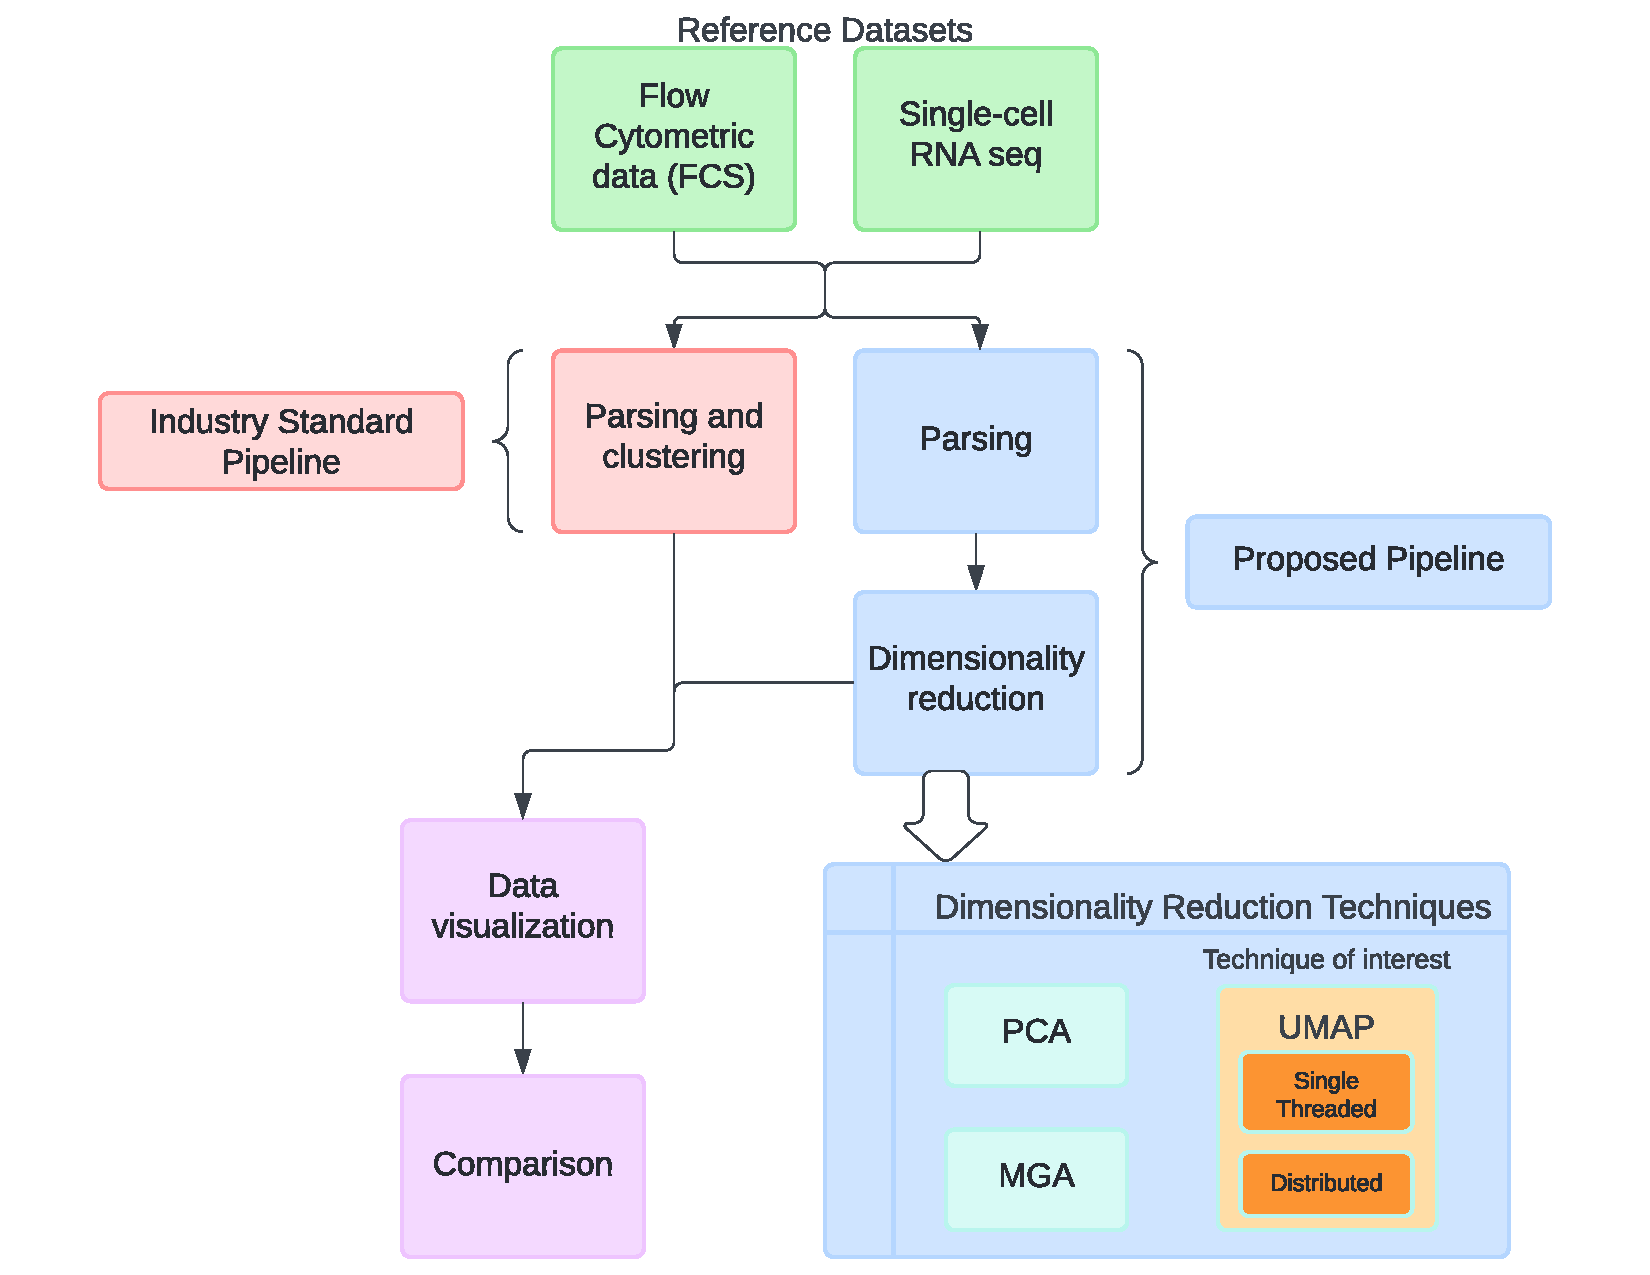
\includegraphics[width=3.4in]{whpc_data_diagram}
    \caption{Data will originate from 3rd-party reference datasets, be analyzed by our pipeline and a reference pipeline, and then our result will be compared against the reference for accuracy.}
    \label{fig:datadiagram}
  \end{minipage}
  % \begin{minipage}[b]{0.48\linewidth}
  %   \centering
  %   \begin{tabular}[l]{|l l|}
  %     \hline
  %     Resource & Quantity \\
  %     \hline
  %     CPUs & $\geq 2$ \\
  %     GPUs & 2 \\
  %     Storage & 2 TB \\
  %     \hline
  %   \end{tabular}\\
  %   \caption{Resource requirements}
  %   % \parbox{1.5in}{\captionof{table:resources}{Resource requirements}}
  %   \label{table:resources}
  % \end{minipage}
\end{figure}

\begin{table}[h]
  \begin{minipage}[b]{0.48\linewidth}
  \centering
  \begin{tabular}[l]{|l l|}
  \hline
  Resource & Quantity \\
  \hline
  CPUs & $\geq 2$ \\
  GPUs & 2 \\
  Storage & 2 TB \\
  \hline
\end{tabular}\\
\caption{Resource requirements}
% \parbox{1.5in}{\captionof{table:resources}{Resource requirements}}
\label{table:resources}
\end{minipage}
\end{table}


\newgeometry{}
\printbibliography
\end{document}
